\documentclass[tikz, border=2pt]{standalone}
\usepackage{amsmath}

\begin{document}
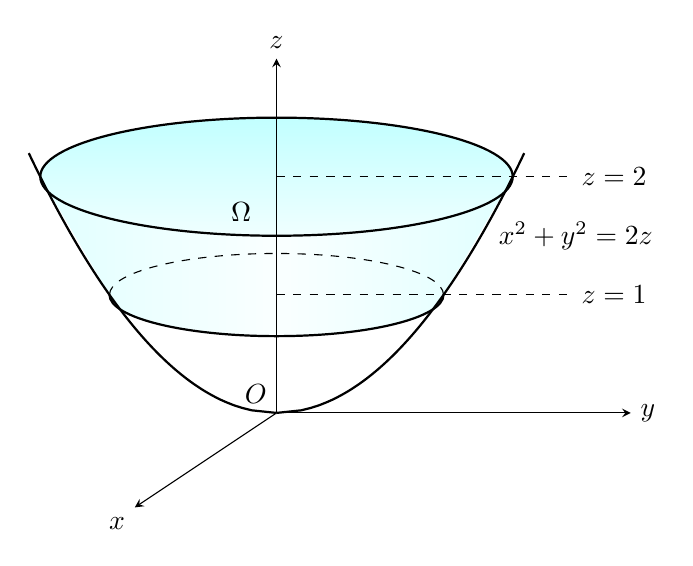
\begin{tikzpicture}[scale=1.5, >=stealth]
    % 1. 绘制侧面阴影 (使用标准的 left color 和 right color)
    \shade[left color=cyan!30, right color=cyan!30, middle color=cyan!5, opacity=0.4]
    (-2,2) arc (180:360:2 and 0.5) -- (1.414,1) arc (360:180:1.414 and 0.35) -- cycle;

    % 2. 绘制顶面圆
    \shade[top color=cyan!40, bottom color=cyan!10, opacity=0.6]
    (0,2) ellipse (2 and 0.5);
    \draw[thick] (0,2) ellipse (2 and 0.5);

    % 3. 画坐标轴
    \draw[->] (0,0) -- (3,0) node[right] {$y$};
    \draw[->] (0,0) -- (0,3) node[above] {$z$};
    \draw[->] (0,0) -- (-1.2,-0.8) node[below left] {$x$};

    % 4. 画抛物面轮廓 (修复点：使用 sqrt 而非 \sqrt)
    \draw[thick, domain=0:2.2, samples=100] plot ({sqrt(2*\x)}, \x);
    \draw[thick, domain=0:2.2, samples=100] plot ({-sqrt(2*\x)}, \x);
    \node[right] at (1.8, 1.5) {$x^2+y^2=2z$};

    % 5. 画 z=1 的截面圆
    \draw[dashed] (1.414,1) arc (0:180:1.414 and 0.35);
    \draw[thick] (1.414,1) arc (0:-180:1.414 and 0.35);
    \draw[dashed] (0,1) -- (2.5,1) node[right] {$z=1$};
    \draw[dashed] (0,2) -- (2.5,2) node[right] {$z=2$};

    % 6. 标注
    \node at (-0.3, 1.7) {$\Omega$};
    \node[above left] at (0,0) {$O$};
\end{tikzpicture}
\end{document}